\section{Geometric realization and dimensional transport}\label{sec:realization}
\subsection{Three tiers of relation}
For a state $x$ there are three nested layers of arithmetic relation: the relations of the lattice $\Lambda_b$ (arithmetic availability), the primitive relations $\Gr_q(x)$, and the \emph{realised moves}, the edges of $\Kmove(x)$, which are pairs of occurrences present in $D(x)$. \cref{fig:possible} depicts the layers; what is proved about each is collected in \cref{prop:P3}.

\subsection{An abstract minimality principle}
\begin{definition}
Let $(P,\prec)$ be a strict partial order and $X\subseteq P$. Put $\min_\prec X=\{g\in X:\ \nexists\,x\in X,\ x\prec g\}$.
\end{definition}
\begin{lemma}[monotone minimality]\label{lem:minimal}
If $X\subseteq X'\subseteq P$ and $g\in\min X$, then $g\in\min X'$ iff no element of $X'\setminus X$ lies below $g$. In particular, if $X_0\subseteq X_1\subseteq\cdots$ and $g\in\min X_{n_0}$, the set $\{n\ge n_0:g\in\min X_n\}$ is an initial segment of $\{n_0,n_0+1,\dots\}$.
\end{lemma}
\begin{proof}
$g\in X'$. An element of $X'$ below $g$ lies either in $X$, impossible by minimality in $X$, or in $X'\setminus X$. For the second claim, if $g\notin\min X_n$ then some $z\in X_n$, $z\prec g$, which stays in $X_{n'}$ for $n'\ge n$.
\end{proof}
\noindent Two instances occur in the sources. (I) Paper~I: $P$ is a lattice with the conformal order $\sqsubseteq$ on integer vectors, $X=\Lambda\setminus\{0\}$, $\min X=\Gr(\Lambda)$; \Src{I}{thm:P2T2} says $g\in\Gr_q(\Lambda')$ iff $g\in\Lambda'$ and no $v\in\Lambda'\setminus\{0,g\}$ satisfies $v\sqsubseteq g$, which is the lemma for $X=\Lambda$, $X'=\Lambda'$ when $\Lambda\subseteq\Lambda'$. (II) Paper~III: for a fixed pair $e=\{u,v\}$ with $\gcd(u,v)>1$ let $P=\{e\}\cup\bigl(I(u,v)\setminus\{u,v\}\bigr)$ with $z\prec e$ for every $z\ne e$, and $X_n=\{e\}\cup(D_n\cap I(u,v)\setminus\{u,v\})$. Then $e\in\min X_n$ iff $D_n\cap(I(u,v)\setminus\{u,v\})=\emptyset$, which by \Src{III}{thm:A5T31} is the condition for $e$ to be an edge once $u,v\in D_n$. The two instances share only the logical shape of the criterion; the ambient sets are different.

\begin{proposition}[\SIV{3}: arithmetic availability versus geometric realization]\label{prop:P3}\status{new, proved; (c),(d) cited}
Let $x_n=C^n(x)$ and $D_n=D(x_n)$.
\begin{enumerate}[label=(\alph*),itemsep=1pt]
\item \emph{Availability of vertices is monotone.} If $u,v\in D_n$ then $u,v\in D_{n'}$ for all $n'\ge n$.
\item \emph{Realisation windows.} For $u,v\in\bigcup_nD_n$, $u\ne v$, let $a(u)=\min\{n:u\in D_n\}$ and $p(u,v)=\min\{n:\ D_n\cap(I(u,v)\setminus\{u,v\})\ne\emptyset\}$ (the first time the interval is pierced by an occurrence; $\infty$ if never; note $1\in I(u,v)$ only if $\gcd(u,v)=1$). Then $\{u,v\}$ is an edge of $\Kmove(x_n)$ iff $\max(a(u),a(v))\le n<p(u,v)$ and, when $\gcd(u,v)=1$, never. In particular the set of times at which a fixed pair is a realised move is an interval of consecutive integers (possibly empty): an edge that disappears never returns.
\item \emph{Availability does not imply a primitive relation is realised.} For $k\ge2$ and the family of \Src{III}{thm:A4T1} the relation $e_i-e_j$ is primitive at $x=P^2/\ell$ (with $D(x)=\{P\}$) and has no pair of fibre points, hence is not realised; it is realised at $y=(Pq)^2/\ell$.
\item \emph{Occurrence inclusion does not control primitive persistence} (\Src{I}{thm:laws}, law L1), whereas persistence of a realised move is controlled by $D$ as in (b).
\end{enumerate}
\end{proposition}
\begin{proof}
(a) is \cref{lem:M-cited}. (b) By \cref{thm:A5T31-cited} below, $\{u,v\}$ is an edge of $\Kmove(x_n)$ iff $u,v\in D_n$ and $I(u,v)\cap(D_n\cup\{1\})=\{u,v\}$. If $\gcd(u,v)=1$ then $1\in I(u,v)\setminus\{u,v\}$ (as $u,v\ge2$), so there is never an edge. If $\gcd(u,v)>1$ then $1\notin I(u,v)$ and the condition is $u,v\in D_n$ and $D_n\cap(I(u,v)\setminus\{u,v\})=\emptyset$, i.e.\ $n\ge\max(a(u),a(v))$ and $n<p(u,v)$ by monotonicity of $D_n$. (c), (d) are cited.
\end{proof}
\begin{theorem}[divisor-interval rule; \Src{III}{thm:A5T31}]\label{thm:A5T31-cited}
Distinct $u,v\in D(x)$ are joined by an edge of $\Kmove(x)$ iff $I(u,v)\cap(D\cup\{1\})=\{u,v\}$.
\end{theorem}
\begin{corollary}[answer to S4, structural part]\label{cor:S4}
The persistence criterion for primitive relations in Paper~I (\Src{I}{thm:P2T2}) and the edge-loss criterion in Paper~III (\Src{III}{thm:A5T31}) are instances of \cref{lem:minimal}, with the ambient orders the conformal order on a lattice and the divisor-interval order on $D$ respectively. An implication from one to the other would need an identification of the two ambient sets; this is open (O7) and is \emph{not} claimed.
\end{corollary}
\begin{figure}[t]\centering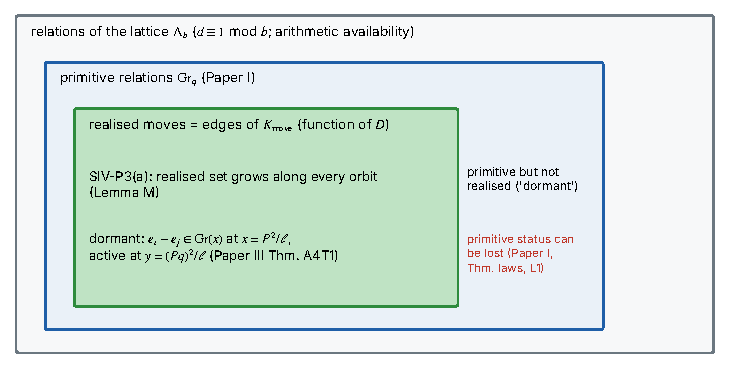
\includegraphics[width=\linewidth]{fig07_possible_vs_realised.pdf}
\caption{\textbf{Arithmetic possibility versus geometric realization.} The relation lattice contains the primitive relations, which contain what is realised as moves of $\Kmove$; the realised set is a function of $D$ and grows along orbits (\cref{prop:P3}(a)), primitive status can be lost. \emph{Schematic of containments; cited exact examples are named.}}\label{fig:possible}\end{figure}

\subsection{The dimensional boundary of transport}
Paper~I proves that for lattices $\Lambda\subseteq\Lambda'$ in rank two the realised union of cells is monotone (\Src{I}{thm:planar}) and that this fails in rank three without a free coordinate (\Src{I}{thm:C1}), with a corner-cube criterion (\Src{I}{thm:corner}) and a slab description when a free coordinate exists (\Src{I}{thm:slab-i}). These statements are about lattice transport, and the relation to occurrence geometry is through \cref{prop:P3}(c),(d): occurrence inclusion is not a lattice inclusion. Finally, abstract loss of a cell does not mean loss from the realised union (\Src{I}{prop:topology}, specimen $21^8/5\to21^8/4$: abstract Betti numbers $(1,5,0)\to(1,2,6)$, realised $(1,2,0)\to(1,0,0)$).

\noindent\Cref{fig:dim} shows planar preservation and three-dimensional failure.

\begin{figure}[t]\centering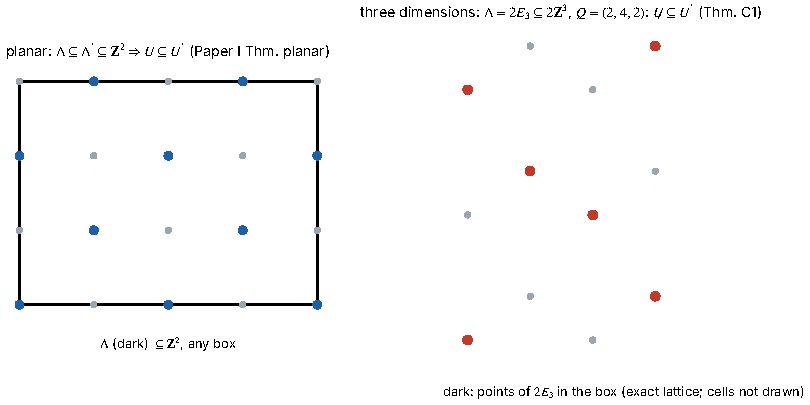
\includegraphics[width=\linewidth]{fig08_planar_vs_3d.pdf}
\caption{\textbf{Planar preservation and three-dimensional failure.} Left: \Src{I}{thm:planar}. Right: \Src{I}{thm:C1} with $\Lambda=2E_3\subseteq2\mathbf{Z}^3$ and box $(2,4,2)$. \emph{Theorem-level schematic: lattice points are exact, cells are not drawn.}}\label{fig:dim}\end{figure}

\noindent\Cref{fig:abs} shows abstract cell loss versus realised geometric containment.

\begin{figure}[t]\centering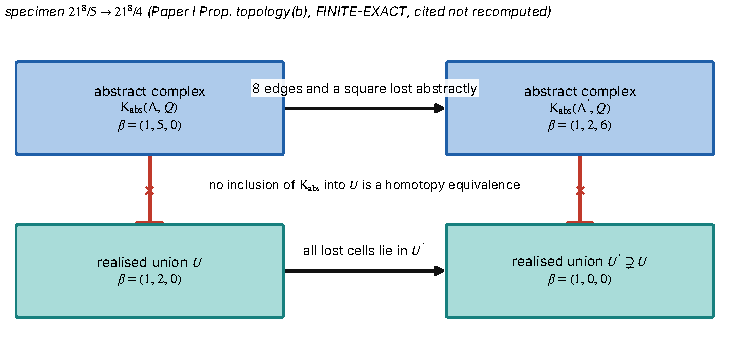
\includegraphics[width=\linewidth]{fig09_abstract_vs_realised.pdf}
\caption{\textbf{Abstract cell loss versus realised geometric containment.} For the planar specimen of \Src{I}{prop:topology}(b) the abstract complex loses cells while the realised union grows. \emph{Finite-exact values quoted from Paper~I, not recomputed.}}\label{fig:abs}\end{figure}
